\documentclass[11pt]{article}

\usepackage{sectsty}
\usepackage{graphicx}
\usepackage{xcolor}
\usepackage{setspace}
\usepackage{hyperref}
\usepackage{gensymb}
\usepackage{amsmath} % for the matrix environments
\usepackage{amsfonts}
\usepackage{amssymb}
\usepackage{cancel}
\usepackage{bbold}
% Margins
\topmargin=-0.90in%-0.45%
\evensidemargin=0in%0in%
\oddsidemargin=0in
\textwidth=7in
\textheight=10.0in
\headsep=0.5in
\onehalfspacing

\title{Epp presentation}
\author{\textbf{\Large Swanith Upadhye, Avik , Apoorve}}
\date{\today}

\begin{document}
	
	\maketitle
	\noindent\hrulefill
	\Large
	
	\section{Partons?}
	\subsection{DIS}
	
	\begin{figure}[h]
		\centering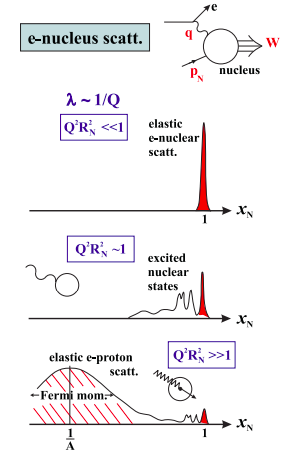
\includegraphics[scale=0.7]{1.png}
		\caption{\centering DIS: Electron - Nucleus cross section vs x \newline \textit{(Alan D. Martin, Acta Physica Polonica B, Vol 39 (2008))}} 
		\label{fig:figure1}
	\end{figure}
	
	The above is the process of scattering of a electron off of a nucleus. 
	\begin{itemize}
		\item q is the 4 momentum of probe
		\item p$_N$ is 4 momentum of Nucleus (M$_N$,$\bar{0}$ if fixed target)
		\item and W(X) is the jet
	\end{itemize}
	
	The invariant mass of the jet (W):
	\[
		W^2 = (p_N + q)^2 = M_N^2 + 2p_N.q + q^2
	\]
	
	Three cases arise depending on the momentum (or more importantly wavelength) of the probe photon. 
		
	\subsubsection{Elastic Regime}
	
	In this regime of CM energies, $\lambda (1/Q) >> R_N $; $W = = M_N$; Hence from the above relation:
	\[
		x = \frac{-q^2}{2p_N.q} = \frac{Q^2}{2M_N\nu} = 1
	\]
	Meaning only at a particular combinations of Q and $\nu$ (probe energies) does the event occur. ($q^2$ is negative for virtual photon not on mass shell; Q$^2$ is positive).
	
	\subsubsection{Inelastic Regime}
	
	Here, the CM energies are such that $\lambda \approx R_N$;
	$W > M_N$
	\[
		\Rightarrow \frac{W^2 - M_N^2}{2p_N.q} = 1 - x  
	\]
	\[
		\Rightarrow x < 1
	\]
	
	The cross section peaks at x$_< 1$ where it may peak at discrete x's corresponding to excited nuclear states, which like higher atomic orbitals have larger radii.
	
	\subsubsection{Deep Inelastic Scattering Regime}
	
	Finally for probe $\lambda << R_N$ or deep (Q$>>M_N$) inelastic(W$>>M_N$) regime:
	\[
		x = \frac{M_p}{M_N} \frac{Q^2}{2M_p \nu} = \frac{1}{A} x_p
	\]
	(Notice Hints of scale, also hints that x becomes fraction of total momentum carried by constituents)
	
	Goes to the elastic scattering regime of nuclear constituents. The peak at x = 1/A is smeared out be momentum of constituents within nucleus. Hence, its a continuum instead of peaks as in Inelelastic case above.
	
	\begin{figure}[h]
		\centering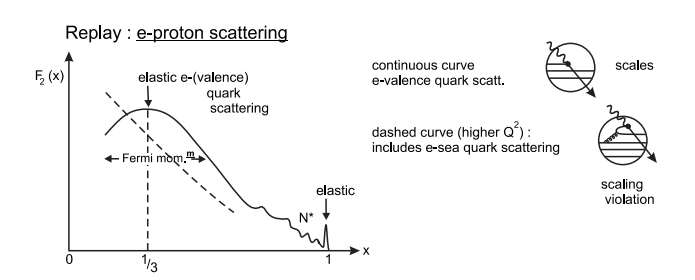
\includegraphics[scale=0.55]{2.png}
		\caption{\centering DIS: Electron - Proton cross section vs x \newline \textit{(Alan D. Martin, Acta Physica Polonica B, Vol 39 (2008))}} 
		\label{fig:figure2}
	\end{figure}
	
	Now similar fate happens for higher Q$^2$ scales, with a constituent peak at 1/3. But no further scaling occurs, just the curve skews towards the dashed line with increased $Q^2$. This is called scaling violation.\\
	Its current understanding is that at large probe energies, gluons are produced which form quark antiquark pairs. Hence large number of constituents are formed, each which carry a smaller momentum fraction x.
	
	\begin{figure}[h]
		\centering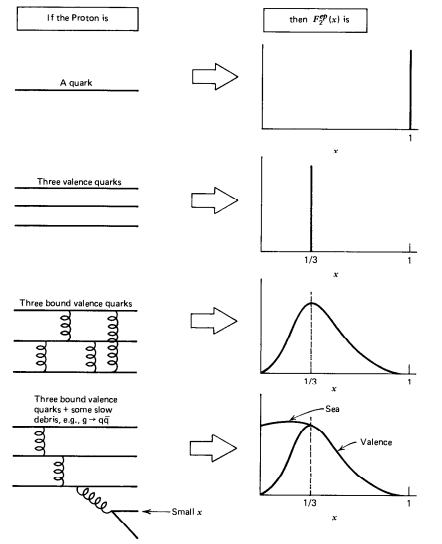
\includegraphics[scale=0.59]{3.png}
		\caption{\centering Scaling and Violation \textit{Halzen and Martin, Quarks and Leptons}}
		\label{fig:figure3}
	\end{figure}
	
	\subsection{Form factors}
	
	The above phenomenon is understood more formally in terms of form factors, as they appear in differential cross sections.\\
	Recall, for point fermion electromagnetic and elastic scattering:
	\[
		\frac{d\sigma}{d\Omega}\vline_{e\mu - e\mu} \propto \{\cos^2\frac{\theta}{2} - \frac{q^2}{2m} \sin^2\frac{\theta}{2}\}\delta(\nu + \frac{q^2}{2m})
	\]
	For extended object elastic scattering:
	\[
		\frac{d\sigma}{d\Omega}\vline_{ep - ep} \propto \{\frac{G_E^2 + \tau G_M^2}{1+\tau}\cos^2 \frac{\theta}{2} + 2\tau G_M^2 \sin^2\frac{\theta}{2}\}\delta(\nu + \frac{q^2}{2M})
	\]
	\(\{\tau = -q^2/ 4M^2\}\)\\
	For Inelastic scattering of extended objects:
	\[
			\frac{d\sigma}{d\Omega}\vline_{ep - eX} \propto \{W_2(\nu, q^2)\cos^2\frac{\theta}{2} + 2W_1(\nu, q^2) \sin^2\frac{\theta}{2}\}
	\]
	
	What happens that for as $Q^2$ goes higher
	\[
	\begin{bmatrix}
		W_1(\nu, Q^2)\\ W_2(\nu, Q^2)   
	\end{bmatrix} \rightarrow
	\Sigma_{i}\frac{mi}{M}\begin{bmatrix}
	\frac{Q^2}{2m_i}\delta(\nu-\frac{Q^2}{2m_i^2})\\ \delta(\nu - \frac{Q^2}{2m_i^2})   
	\end{bmatrix}
	\]
	(where the sum is over constituents)
	
	
	
	\section{PDFs ?}
	
	
	
	
\end{document}